\documentclass[12pt,a4paper]{article}
\usepackage[width=.75\textwidth]{caption}
\usepackage{graphicx}
\usepackage{authblk}
\usepackage{amsmath}
\usepackage{amsfonts}
\usepackage{braket}
\usepackage{epigraph}
%\usepackage{mathrsfs}
\usepackage[mathscr]{euscript}
\usepackage[top=2cm, bottom=2cm, left=2cm, right=2cm]{geometry}
\usepackage{fancyhdr}

\setlength{\epigraphwidth}{0.8\textwidth}

\pagestyle{fancy}
\begin{document}

%title and author details
\title{The Unruh Effect as Holographic Thrust}
\author[1]{Kevin Player\footnote{kjplaye@gmail.com}}

\maketitle

\epigraph{The Unruh effect tells us that what we call particles is really just a matter of perspective.}{Lee Smolin}


\abstract{We outline the holographic scenario from entropic gravity and additionally consider the dynamics of the holographic screen itself in an accelerating frame.  We consider the case where the screen's acceleration is due to mass/energy joining with the screen, increasing the entropy of the screen.  Finally, we consider the field theoretic picture where Unruh radiation was initially uncovered.  In both cases, we illustrate the Unruh effect through the utilization of thrust.}

\section{The Holographic Scenario}
We first recall the setup outlined in \cite{entropic}. Consider a holographic screen $\mathscr{S}$ with entropy $S$.  Let there be a test particle which is a single wavelength $\Delta x$ away from $\mathscr{S}$.  Following Bekenstein \cite{bekenstein}, we can regard the particle to be simultaneously near and on the screen.

Let the screen have energy $E_\mathscr{S}$ and mass $M_\mathscr{S}$.  Suppose that the holographic screen is being propelled by a stream of photons in place of the test particle.  We want to see how the dynamics of the photons affects the dynamics and information carried by the screen.

\begin{figure}[h]
\centering
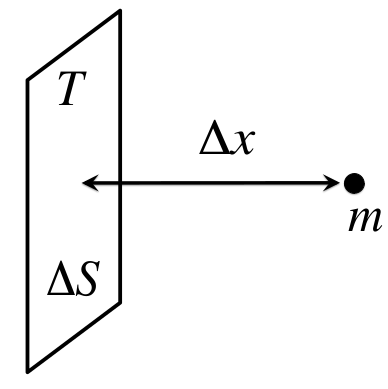
\includegraphics[scale=1.2]{screen.png}
\caption{This figure was copied from \cite{entropic}.  A test particle with mass $m$ and Compton wavelength $\Delta x$ is being absorbed into the holographic screen.  In this note, we replace the test particle with a single photon.}
\label{fig:x cubed graph}
\end{figure}
There are some complementary notions of ``emergence'' that we inherit from \cite{entropic}.  A third notion, item 3, that we supply here is the time-reversal of matter/energy emerging from the screen.
\begin{enumerate}
  \item The usual thermodynamic emergence of macrostate variables (such as temperature) from microstate variables (energies of individual particles).  This includes the emergence of Newton's laws and entropic gravity.
  \item The emergence of ``new'' space-time beyond holographic screens, treating screens like stretched horizons, far away from the actual event horizons.  The existence of a foliation of screens where test particles move from screen to screen.
  \item Known matter/energy in front of the screen passes to unknown matter/energy on the screen. The matter/energy in front of the screen has known information.  When passing into the screen, the information is thermalized, and becomes unknown.
\end{enumerate}
The information theoretic notions of emergence will be discussed in more detail in terms of Landauer's language in the next section.

\section{Landauer Limit}
We want to keep track of the information corresponding to degrees of freedom on the screen. It is interesting to compare this situation with the limiting case of Landauer \cite{landauer}.  The situation can be made to be identical by letting the holographic screen be the separation between the system and the heat bath (between the known and the unknown).  Forgetting (or learning) information is the same thing as letting the information ``join the screen'' (``emerge from the screen'' resp.).

We pause to note that there is nothing canonical about choosing a bit to express this information.  For instance, Landauer considered logical gates and as an example, we briefly consider the AND gate on two unbiased bits of input.  The output is a bit, but it is biased, and so it carries less than one bit of information.  The AND gate actually forgets more than a bit\footnote{It actually forgets around 1.19 bits}.  All of this is to say that the choice of $\Delta S$ is far from obvious.

Consider the case where a single photon of energy $E_p$ is joining the screen.  The change of information, per photon, will be a constant.  It is not given by $k\ln(2)$, from a bit, but by another number
\[
  \Delta S = 4 \pi ^ 2 k.
\]
There is nothing mysterious here; we pick this constant so that we will match the constant in Unruh radiation.

\section{Information Theoretic Unruh Effect}

We will derive the Unruh temperature equation from the information change of an accelerating screen due to the thrust of photons. For a single photon in the stream, consider the Planck relation for the energy and frequency of the screen
\[
  E_\mathscr{S} = h f_\mathscr{S} = \frac{h}{\Delta t}
\]
where $\Delta t$ is the period of $\mathscr{S}$. Let $a$ be the acceleration due to the photon which we also write as $a = \Delta v / \Delta t$.  Let $p$ be the momentum of the photon, $E_p$ its energy, and we equate the momenta $p_\mathscr{S}$ = $p_p$ = $p$ for an elastic collision with the screen.  Then
\[
  a M_\mathscr{S} \Delta t = M_\mathscr{S}  \Delta v = p = E_p / c
  \]
and setting a temperature $T$, with respect to $E_p$, we get
\[
  \frac{4 \pi^2 k}{h} E_\mathscr{S} = \frac{\Delta S}{\Delta t} = \frac{E_p}{T \Delta t} = \frac{ca M_\mathscr{S}}{T} = \frac{aE_\mathscr{S}}{cT}
\]
and canceling $E_\mathscr{S}$ we derive the Unruh temperature \cite{unruh}
\[
T = \frac{h}{4\pi^2k c} a
\]

\section{Field Theoretic Considerations}
Let $\hbar$ = c = 1.
\subsection{Rindler and Minkowski Modes Review}
Much of this section including notation and conventions are drawn directly from the overview \cite{Frodden}, from the original source \cite{unruh}, and from \cite{beisert}.

Consider a $(1,1)$-dimensional spacetime\footnote{It is not useful to consider the full $(1,3)$-dimensional case, so we stick to the dimensions where the linear acceleration boosts are taking place -- $t$ and $z$.} $(t,z)$ with ``event horizon'' coordinates $u = -t + z$ and $v = -t - z$.   Any function of purely $u$, $f(u)$, is made up of Minkowski modes that are constant on $v$.  That is they are given by a 1-dimensional Fourier expansion
\[
f(u) = \frac{1}{2\pi} \int{e^{i p_u u} \hat{f}(p_u) dp_u}.
\]
The same is true for $v$, $g(v)$, $p_v$, and $\hat{g}(v)$.  The full 2-dimensional transform of combinations of $f$ and $g$ is a linear combination of $\hat{f}(p_u) \delta(p_v)$ and $\hat{g}(p_v) \delta(p_u)$.  These are supported on the massless shell --- ``the momentum light cone''.

\begin{figure}[h]
\centering
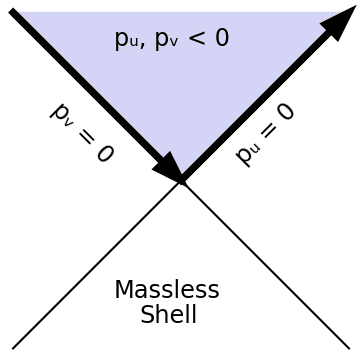
\includegraphics[scale=1.0]{massless_shell.png}
\caption{}
\label{masslessshell}
\end{figure}


Let $W$ be the $z>|t|$ Rindler wedge with coordinates
\[
t = \frac{1}{a}e^{a\xi}\sinh{(a\eta)}
\]
\[
z = \frac{1}{a}e^{a\xi}\cosh{(a\eta)}
\]
where $a>0$ is an acceleration parameter (see Figure \ref{rindlerw}).

\begin{figure}[h]
\centering
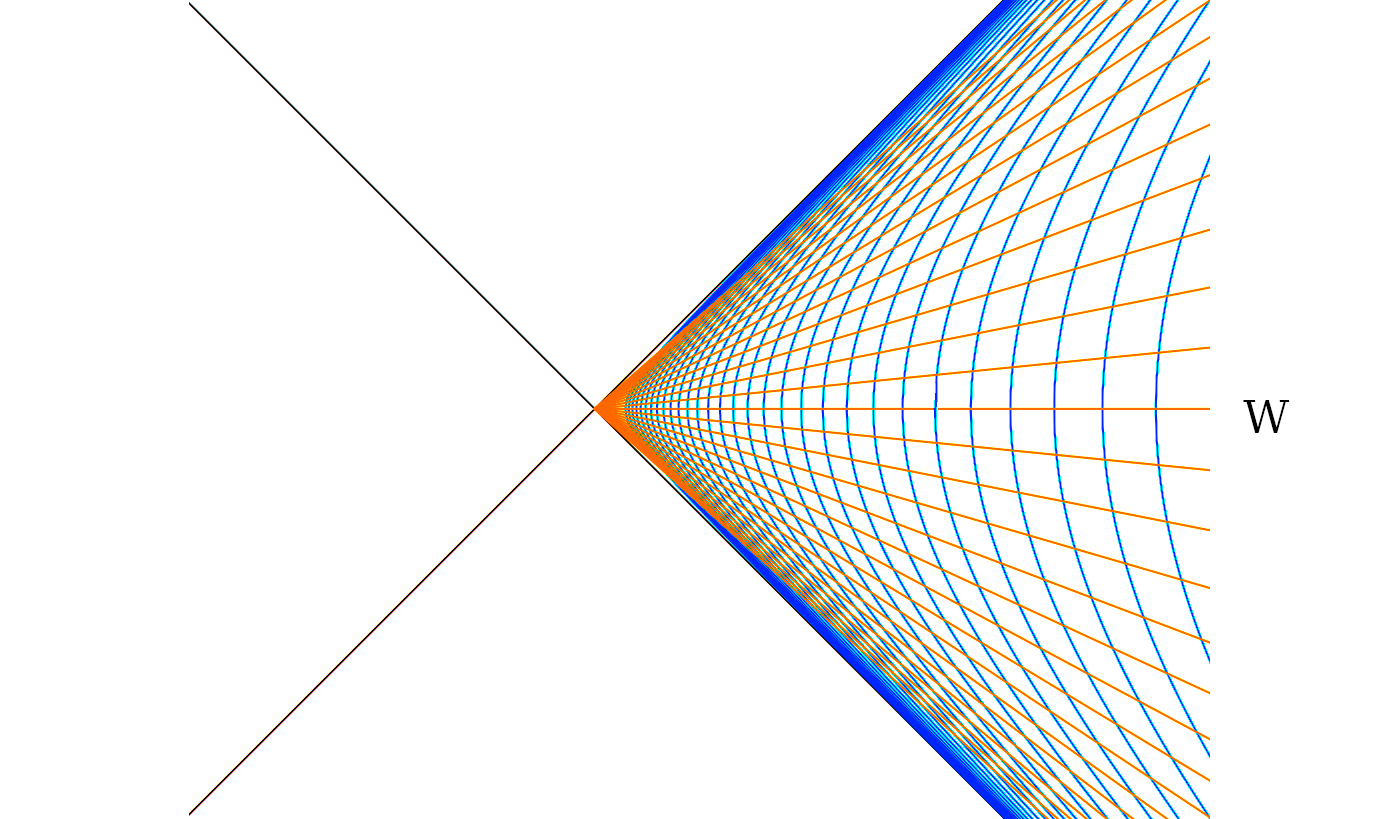
\includegraphics[scale=0.4]{rindler_w.png}
\caption{Rindler wedge $W$ on the right.}
\label{rindlerw}
\end{figure}


For wave number $k$ and positive frequency $\omega_k$ consider the functions
\[
h^{(u)}_k = \frac{e^{\frac{\pi \omega_k}{2a}} {(au)}^{\frac{i\omega_k}{a}}}{ \sqrt{2\sinh\left(\frac{\pi\omega_k}{a}\right)} }
\]
\[
h^{(v)}_k = \frac{e^{\frac{\pi \omega_k}{2a}} {(av)}^{\frac{i\omega_k}{a}}}{ \sqrt{2\sinh\left(\frac{\pi\omega_k}{a}\right)} }
\]
The scalar field in Rindler curved space has modes
\[
 r_k = \frac{1}{\sqrt{4 \pi \omega_k}} e^{-i(\omega_k \eta -k \xi)}
\]
which can be written as combinations of the ``event horizon'' modes
x\[
e^\frac{\pi\omega_k}{2a} h^{(u)}_k - e^{-\frac{\pi\omega_k}{2a}} h^{(v)}_k  = \sqrt{2 \sinh \left({\frac{\pi\omega_k}{a}}\right)} r_k
\]
Unlike the Rindler mode, the event horizon modes extend analytically from $W$ to all of spacetime.


When we switch between $h_k$ and the usual Minkowski bases we find that the Minkowski vacuum has excitations coming from the Rindler modes.  More specifically, there is a positive particle number vacuum expectation of
\begin{equation}
\label{radeq}
\frac{1}{e^{\frac{2 \pi \omega_k}{a}}-1}
\end{equation}
which is interpreted as (Unruh) radiation \cite{unruh}.

\subsection{Fourier Transform of the Sources}

Let $\phi$ be a scalar field in the flat $(1,1)$-dimensional Minkowski spacetime\footnote{Note that we only consider the scalar case.  Generalization to other fields is straightforward and does not add any intuition to the presentation.}.  We will consider $h^{(u)}_k$ and $h^{(u)}_k$ as driving $W$-event horizon sources
\begin{equation}
\label{ab}
\rho = \alpha h^{(u)}_k + \beta h^{(v)}_k.
\end{equation}
with positive real convex combination $(\alpha + \beta) = 1$.
The drivers $h^{(u)}_k$ and $h^{(v)}_k$ are functions $f(u)$ of the past $W$-horizon and $g(v)$ of the future $W$-horizon respectively.  Both generate excitations, which we identify with absorption and emission thrusts respectively.


The source can originate from a coupling term, $\rho \phi$, added to the Lagrangian.
\[
\mathscr{L}_{driven} = \mathscr{L}_{original} + \rho\phi 
\]
This leads to an inhomogeneous Klein-Gordon equation
\[
(\Box + m^2) \phi = \rho
\]
as presented in \cite{beisert}\footnote{In \cite{beisert} it is assumed that the source is only active for a finite amount of time.  We let $\rho$ be active for all time.  The argument in \cite{beisert} seem to be adaptable to $\rho$.}

We want to integrate $\rho$ on shell in momentum space, which for a massless source is the positive energy part of the massless shell.  The two positive energy ``horizons'' border $p_u <= 0$ and $p_v <= 0$, see Figure \ref{masslessshell}.  Proceeding to take the Fourier transform of the function $f(u)$\footnote{WLOG since $g(v)$ is of the same form.}, we drop $p_u$ to just $p$ for the time being to increase legibility.  We will continue to assume that $\omega_k$ and $a$ are positive. Define the kernel
\[
  A = e^{-i p u} (au)^\frac{i\omega_k}{a} du
\]
and then we have
\begin{equation}
\label{finalnorm}
  \hat{f}(\rho_U) =  \frac{e^{\frac{\pi \omega_k}{2a}}}{\sqrt{2 \sinh \left({\frac{\pi\omega_k}{a}}\right)}}  \int_{-\infty}^\infty A
\end{equation}
where $L=\int_{-\infty}^0 A$ and $R=\int_0^\infty A$ are the left and right sides of the total integral $L + R$.

We rewrite the integrals using a complex changes of variables, $s$ = $ipu$, and contour integrals.

\begin{figure}[h]
\centering
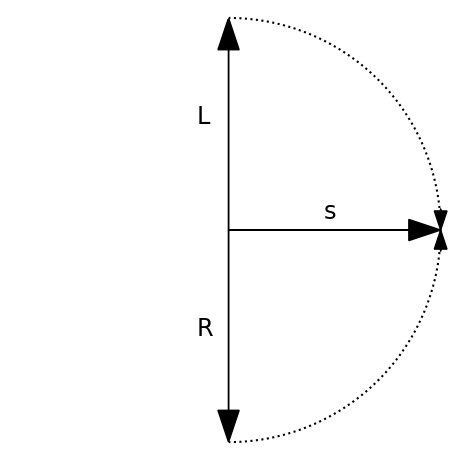
\includegraphics[scale=0.6]{contour.png}
\caption{Using contours with large radius we convert the $L$ integral that goes to $i\infty$, and the $R$ integral that goes to $-i\infty$, to integrals with $s$ going to real $\infty$.}
\label{fig:x cubed graph}
\end{figure}


The $L$ integral for real $p<0$ is
\[
\begin{split}
  L(p) & = -\int_0^{i\infty} \left(\frac{ias}{-p}\right)^\frac{i\omega_k}{a} \left(\frac{i}{-p}\right)ds \\
  & = \frac{-i}{a} \left(\frac{a}{-p}\right)^{\frac{i\omega_k}{a} + 1} \int_0^\infty \left(is\right) ^ \frac{i\omega_k}{a} e^{-s} ds \\
  & = \frac{-i}{a} \left(\frac{a}{-p}\right)^{\frac{i\omega_k}{a} + 1} \Gamma\left(\frac{i\omega_k}{a} + 1\right) e^{-\frac{\pi \omega_k}{2a}} \\
  & = \frac{1}{2} \Gamma\left(\frac{i\omega_k}{a} + 1\right) e^{-\frac{\pi \omega_k}{2a}} B(p)\\
\end{split}
\]
where
\[
B(p) = \frac{-2i}{a} \left(\frac{a}{-p}\right)^{\frac{i\omega_k}{a} + 1} 
\]
is as shown.  This is using a large radius contour which rotates the endpoint 90 degrees clockwise.

The same calculation for $R$ is done using a counter-clockwise contour this time.
\[
\begin{split}
  R(p) = \frac{1}{2}\Gamma\left(\frac{i\omega_k}{a} + 1\right) e^{-\frac{\pi \omega_k}{2a}} B(p)
\end{split}
\]

We get back to $h_k^{(u)}$ and apply the normalization from (\ref{finalnorm})
\[
\hat{h_k}^{(u)}(p_u) = \frac{e^{\frac{\pi \omega_k}{2a}}}{\sqrt{2 \sinh \left({\frac{\pi\omega_k}{a}}\right)}}  ( L(p_u) + R(p_u) )
\]
So
\begin{equation}
\label{fourier}
\begin{split}
\hat{h_k}^{(u)}(p_u) & = \frac{\Gamma\left(\frac{i\omega_k}{a} + 1\right)}{\sqrt{2 \sinh \left({\frac{\pi\omega_k}{a}}\right)}} B(p_u)\\
\hat{h_k}^{(v)}(p_v) &= \frac{\Gamma\left(\frac{i\omega_k}{a} + 1\right)}{\sqrt{2 \sinh \left({\frac{\pi\omega_k}{a}}\right)}} B(p_u)
\end{split}
\end{equation}
\subsection{Interpretation}
The driving source $\rho$, with mixed absorption and emission thrusts $\alpha$ + $\beta$ = 1, contribute excitations to the scalar field $\phi$. Equations (\ref{ab}) and (\ref{fourier}) let us write down the expected change of energy
\begin{equation}  
  \label{number}
  \begin{split}
    \mathbb{E}[\Delta E] &= \frac{1}{4\pi} \int{|\rho(p)|^2 dp} \\
    &= \frac{\alpha}{4\pi} \int{\left|\hat{h_k}^{(u)}(p_u)\right|^2 dp_u} + \frac{\beta}{4\pi}\int{\left|\hat{h_k}^{(v)}(p_v)\right|^2dp_v} \\
    &= \frac{\left|\Gamma\left(\frac{i\omega_k}{a} + 1\right)\right|^2}{2 \sinh \left({\frac{\pi\omega_k}{a}}\right)} \frac{1}{4\pi} \int{{\left|B(p)\right|^2} dp} \\
    &=  \frac{\left|\Gamma\left(\frac{i\omega_k}{a} + 1\right)\right|^2}{2 \pi a \sinh \left({\frac{\pi\omega_k}{a}}\right)} \int{a/|p|^2 dp}\\  
&=I(\omega_k) P
  \end{split}
\end{equation}
where the integrals are on the positive energy massless shell with contributions from $p_u$ on the left piece and $p_v$ on the right piece.  We factored out $P = \int{a/|p|^2}$ with a remaining $p$ independent positive real coefficient $I(\omega_k)$.

Without being more careful about wave packets we end up with inferred problems --- The integrals do not converge at zero, where $P$ explodes.  But this infinity cancels when we compare the spectral radiances $I(\omega_k)$ to each other.

The magnitude of our Gamma function has known asymptotics \cite[Eq.~5.11.9]{NIST:DLMF}
\[
\left|\Gamma\left(\frac{i\omega_k}{a} + 1\right) \right|^2 \sim \left(\frac{2 \pi \omega_k} {a}\right) e^{-\frac{\pi\omega_k}{a}}
\]
Plugging this into equation (\ref{number}) we find the average thermal energy of the mode, the (1,1) dimensional Planck distribution function, and thus recover the Unruh's radiation spectrum\footnote{Compare to equation (\ref{radeq}) and references \cite{unruh} and \cite{Frodden}.} from a thrust driven field.
\[
\frac{1}{P} \mathbb{E}[\Delta E] = I(\omega_k) \sim \frac{\omega_k}{e^{\frac{2 \pi \omega_k}{a}}-1}
\]

\section{Hawking-Bekenstein Radiation and the Equivalence Principle}

The equivalence principle allows us to transfer linear acceleration conclusions to accelerations due to gravity.  Unruh's temperature maps to a temperature for acceleration due to gravity -- for instance near the event horizon of a black hole\footnote{This leads to the celebrated black hole radiation.  The equivalence principle is used to equate this with Unruh radiation see \cite{unruh}}.  This corresponds to a reference frame which continues to thrust away from a black hole, maintaining a given height.  Thrust that explains Unruh radiation also explains Hawking-Bekenstein radiation.

\section{Acceleration and Observation}
We have seen how acceleration is paired with an accelerating thrust.  Central to this idea is the implicit separation of the accelerated system from the rest of the universe.  We have studied the fanciful holographic screens from entropic gravity, Landauer's principle, and the Rindler horizons.  In all of these cases, there is a separation between the accelerated system that we are a part of $\mathcal{A}$, and the remaining heat bath $\mathcal{H}$.

Suppose we add the particles responsible for the thrust, $\mathcal{T}$, back into to our system.  The resulting larger system,  $\mathcal{B}$ = $\mathcal{A} + \mathcal{T}$, would no longer experience a net acceleration since all of the forces balance out.  This is the essence of Newton's third law.  So the very existence of a nonzero acceleration requires the separation of the system $\mathcal{A}$ from its thrust $\mathcal{T}$.

The physical difference between $\mathcal{A}$ and $\mathcal{B}$ is the thrust $\mathcal{T}$.  In accordance with Landauer, the following transitions are neatly summerized:
\begin{enumerate}
\item A direct application of Landauer's principle, \\ \hspace*{1 in} $\mathcal{B} \rightarrow \mathcal{A}$ corresponds to {\bf ``Forgetting''} $\mathcal{T}$.\\
\item A reverse application of Landauer's principle, \\ \hspace*{1 in} $\mathcal{A} \rightarrow \mathcal{B}$ corresponds to {\bf ``Learning''} $\mathcal{T}$.\\
\end{enumerate}
The 2nd transition is a ``measurable'' in $\mathcal{A}$. This could be a full on apperception by a conscious observer, an interaction with a particle, or just a measurement potential.  The key here is an increase in total information in $\mathcal{A}$.  This is related exactly to an increase in total mass/energy by Landauer's principle.  The 1st transition is not measurable in $\mathcal{A}$, but an opposite, a measurable in $\mathcal{H}$


\section{Conclusion and Prediction}
If we do not account for the thrust required to accelerate a detector, then we recover it instead as a thermal unknown in the vacuum, Unruh radiation.  But, it would seem that we can explain Unruh radiation directly using thrust in the illustrative ways outlined in this paper.  The prediction of this note is that Unruh radiation, separate from thrust, should not appear.

\section{Acknowledgments}
Thanks to Daniel Justice for useful discussions.

\bibliographystyle{ieeetr}
\bibliography{bibliography}

\end{document}
